\documentclass[12pt, a4paper]{article}
\usepackage[utf8]{vietnam}
\usepackage[margin = 2cm]{geometry}
\usepackage{amsmath,amsfonts,amssymb}
\usepackage{indentfirst,enumitem}
\usepackage{graphicx}
\usepackage[font=small,labelfont=bf]{caption}
\usepackage{multicol}
\usepackage{setspace}
\usepackage{hyperref}
\usepackage{listings}
\usepackage{tabularx}
\usepackage{hyperref}
\usepackage[dvipsnames]{xcolor}
\usepackage{scrextend}
\usepackage{comment}
\usepackage{soul}
\usepackage{tikz,tkz-tab}
\usepackage{lscape}
\usepackage{float,lscape}
\usepackage{fancyhdr}
\usepackage{tcolorbox}
\usepackage{titling}
\usepackage{import}
\usepackage{titlesec}
\usepackage{color}
\usepackage{empheq}

%%%%%%%%%%%%%%%%%%%%

\newcommand*\widefbox[1]{\fbox{\hspace{2em}#1\hspace{2em}}} %BOX FOR EQUATION SETUP AND EMQHEQ

\hypersetup{
    colorlinks=true,% make the links colored
}

\pagestyle{fancy}
\fancyhead[r]{Huy Vu}
\fancyhead[c]{\bfseries Electric Circuit Analysis}
\fancyhead[l]{\today}
\renewcommand{\headrulewidth}{0.2pt}
\setlength{\headheight}{15pt}

\begin{document}


\begin{titlepage}
    \centering
    \vspace*{1in}

    {\LARGE \bfseries Introduction to Electric Circuit Analysis}\\[1.5cm]

    {\large Huy Vu}\\[0.5cm]
    {\large Department of Telecomunications Engineering}\\
    {\large Falcuty of Electrical and Electronics Engineering}\\
    {\large Ho Chi Minh City University of Technology}\\[2cm]

    {\large \today}

    \vfill
    \textbf{Thanh pho Ho Chi Minh $-$ 2024}
\end{titlepage}
{
  \hypersetup{linkcolor=[RGB]{236, 16, 145}}
  \tableofcontents
}
\newpage
\section{HỆ THỐNG SỐ ĐẾM - SỐ NHỊ PHÂN}
\subsection{Các hệ thống số đếm:}
\subsubsection{Khái niệm:}
\begin{itemize}
    \item[-] Cơ số (r-radix): là số lượng ký tự chữ số (ký số - digit) sử dụng để biểu diễn trong hệ thống số đếm.
    \item[-] Trọng số (weight): đại lượng biểu diễn cho vị trí của 1 con số trong chuỗi số.\\ \textbf{Trọng số = $\text{Cơ số}^\text{vị trí}$}
    \item[-] Giá trị (value): tính bằng tổng theo trọng số. \textbf{Giá trị = $\sum$ (Ký số $\times$ Trọng số).}
\end{itemize}
\textbf{a. Số thập phân (Decimal): Cơ số $r = 10$.}
\begin{table}[h!]
    \centering
    \begin{tabular}{|c|c|c|c|c|c|c|}
    \hline
    \textbf{4}                                   & \textbf{0}                                   & \textbf{7}                                   & \textbf{.} & \textbf{6}                                        & \textbf{2}                                        & \textbf{5}                                        \\ \hline
    $10^2$                        & $10^1$                        & $10^0$                        & .          & $10^{-1} $                       & $10^{-2}$                        & $10^{-3}$                        \\ 
    $4\times 10^2$ & $0\times 10^1$ & $7\times 10^0$ & .          & $6\times 10^{-1}$ & $2\times 10^{-2}$ & $5\times 10^{-3}$ \\ 
   $ 400 $                                         & $0$                                            & $7$                                            & .          & $0.6$                                               & $0.02$                                              & $0.005$                                             \\ \hline
    \end{tabular}
\end{table}
\[
    400 + 0 + 7 + 0.6 + 0.02 + 0.005 = 407.625
\]
\textbf{b. Số nhị phân (Binary): Cơ số $r=2$.}
\begin{table}[h!]
    \centering
    \begin{tabular}{|c|c|c|c|c|c|c|}
    \hline
    \textbf{1}                                   & \textbf{0}                                   & \textbf{1}                                   & \textbf{.} & \textbf{0}                                        & \textbf{1}                                        & \textbf{1}                                        \\ \hline
    $2^2$                        & $2^1$                        & $2^0$                        & .          & $2^{-1} $                       & $2^{-2}$                        & $2^{-3}$                        \\ 
    $1\times 2^2$ & $0\times 2^1$ & $1\times 2^0$ & .          & $0\times 2^{-1}$ & $1\times 2^{-2}$ & $1\times 2^{-3}$ \\ 
   $ 4 $                                         & $0$                                            & $1$                                            & .          & $0$                                               & $0.25$                                              & $0.125$                                             \\ \hline
    \end{tabular}
\end{table}
\[
    4 + 0 +1+0+0.25+0.125=5.375
\]
\textbf{c. Số thập lục phân (Hexadecimal): Cơ số $r=16$}
\begin{table}[h!]
    \centering
    \begin{tabular}{|c|c|c|c|c|c|c|}
    \hline
    \textbf{5}     & \textbf{A}      & \textbf{0}     & \textbf{.} & \textbf{4}        & \textbf{D}         & \textbf{1}        \\ \hline
    $16^2$         & $16^1$          & $16^0$         & .          & $16^{-1} $        & $16^{-2}$          & $16^{-3}$         \\ 
    $5\times 16^2$ & $10\times 16^1$ & $0\times 16^0$ & .          & $4\times 16^{-1}$ & $13\times 16^{-2}$ & $1\times 16^{-3}$ \\ 
    $ 1280 $       & $160$           & $0$            & .          & $0.25$            & $0.0508$           & $0.002$           \\ \hline
    \end{tabular}
\end{table}
\[
    1280 + 160+0+0.25+0.0508+0.0002 = 1440.301
\]
\subsubsection{Chuyển đổi cơ số:}
\noindent\textbf{a. Từ thập phân sang nhị phân:}
\newpage
\[
  8.625  
\]
\begin{center}
    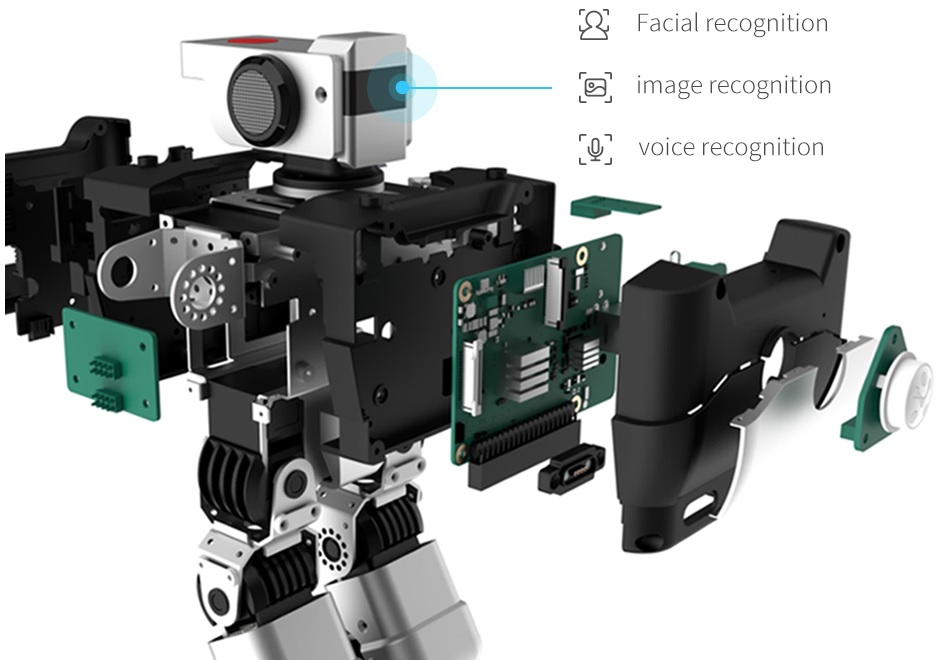
\includegraphics[width = 0.65\textwidth]{./local/image/1.png}
\end{center}
\textbf{b. Từ thập phân sang thập lục phân:}
\[
    1480.4296875
\]
\begin{center}
    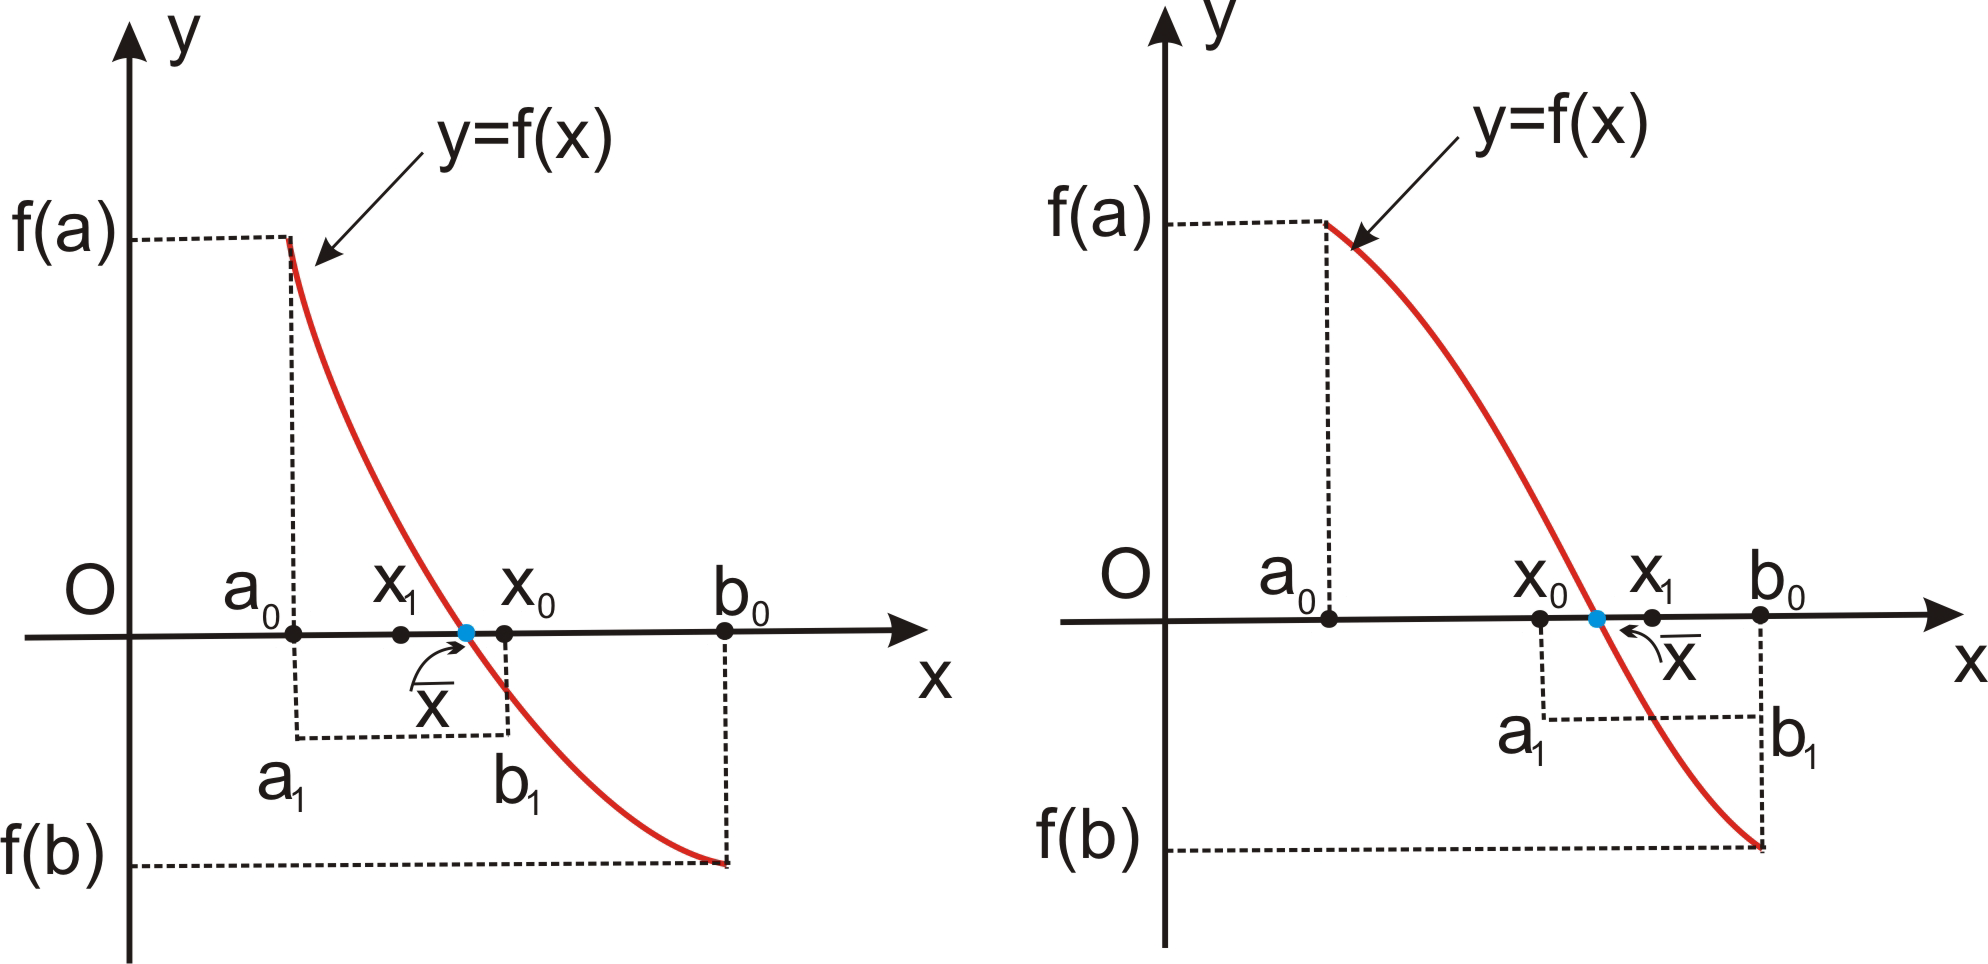
\includegraphics[width = 0.65\textwidth]{./local/image/2.png}
\end{center}
\textbf{c. Từ nhị phân sang thập lục phân}
\begin{center}
    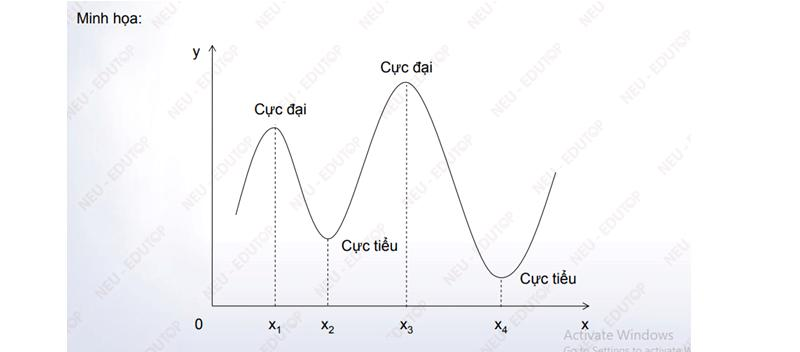
\includegraphics[width = 0.65\textwidth]{./local/image/3.png}
\end{center}
\textbf{d. Từ thập lục phân sang nhị phân}
\begin{center}
    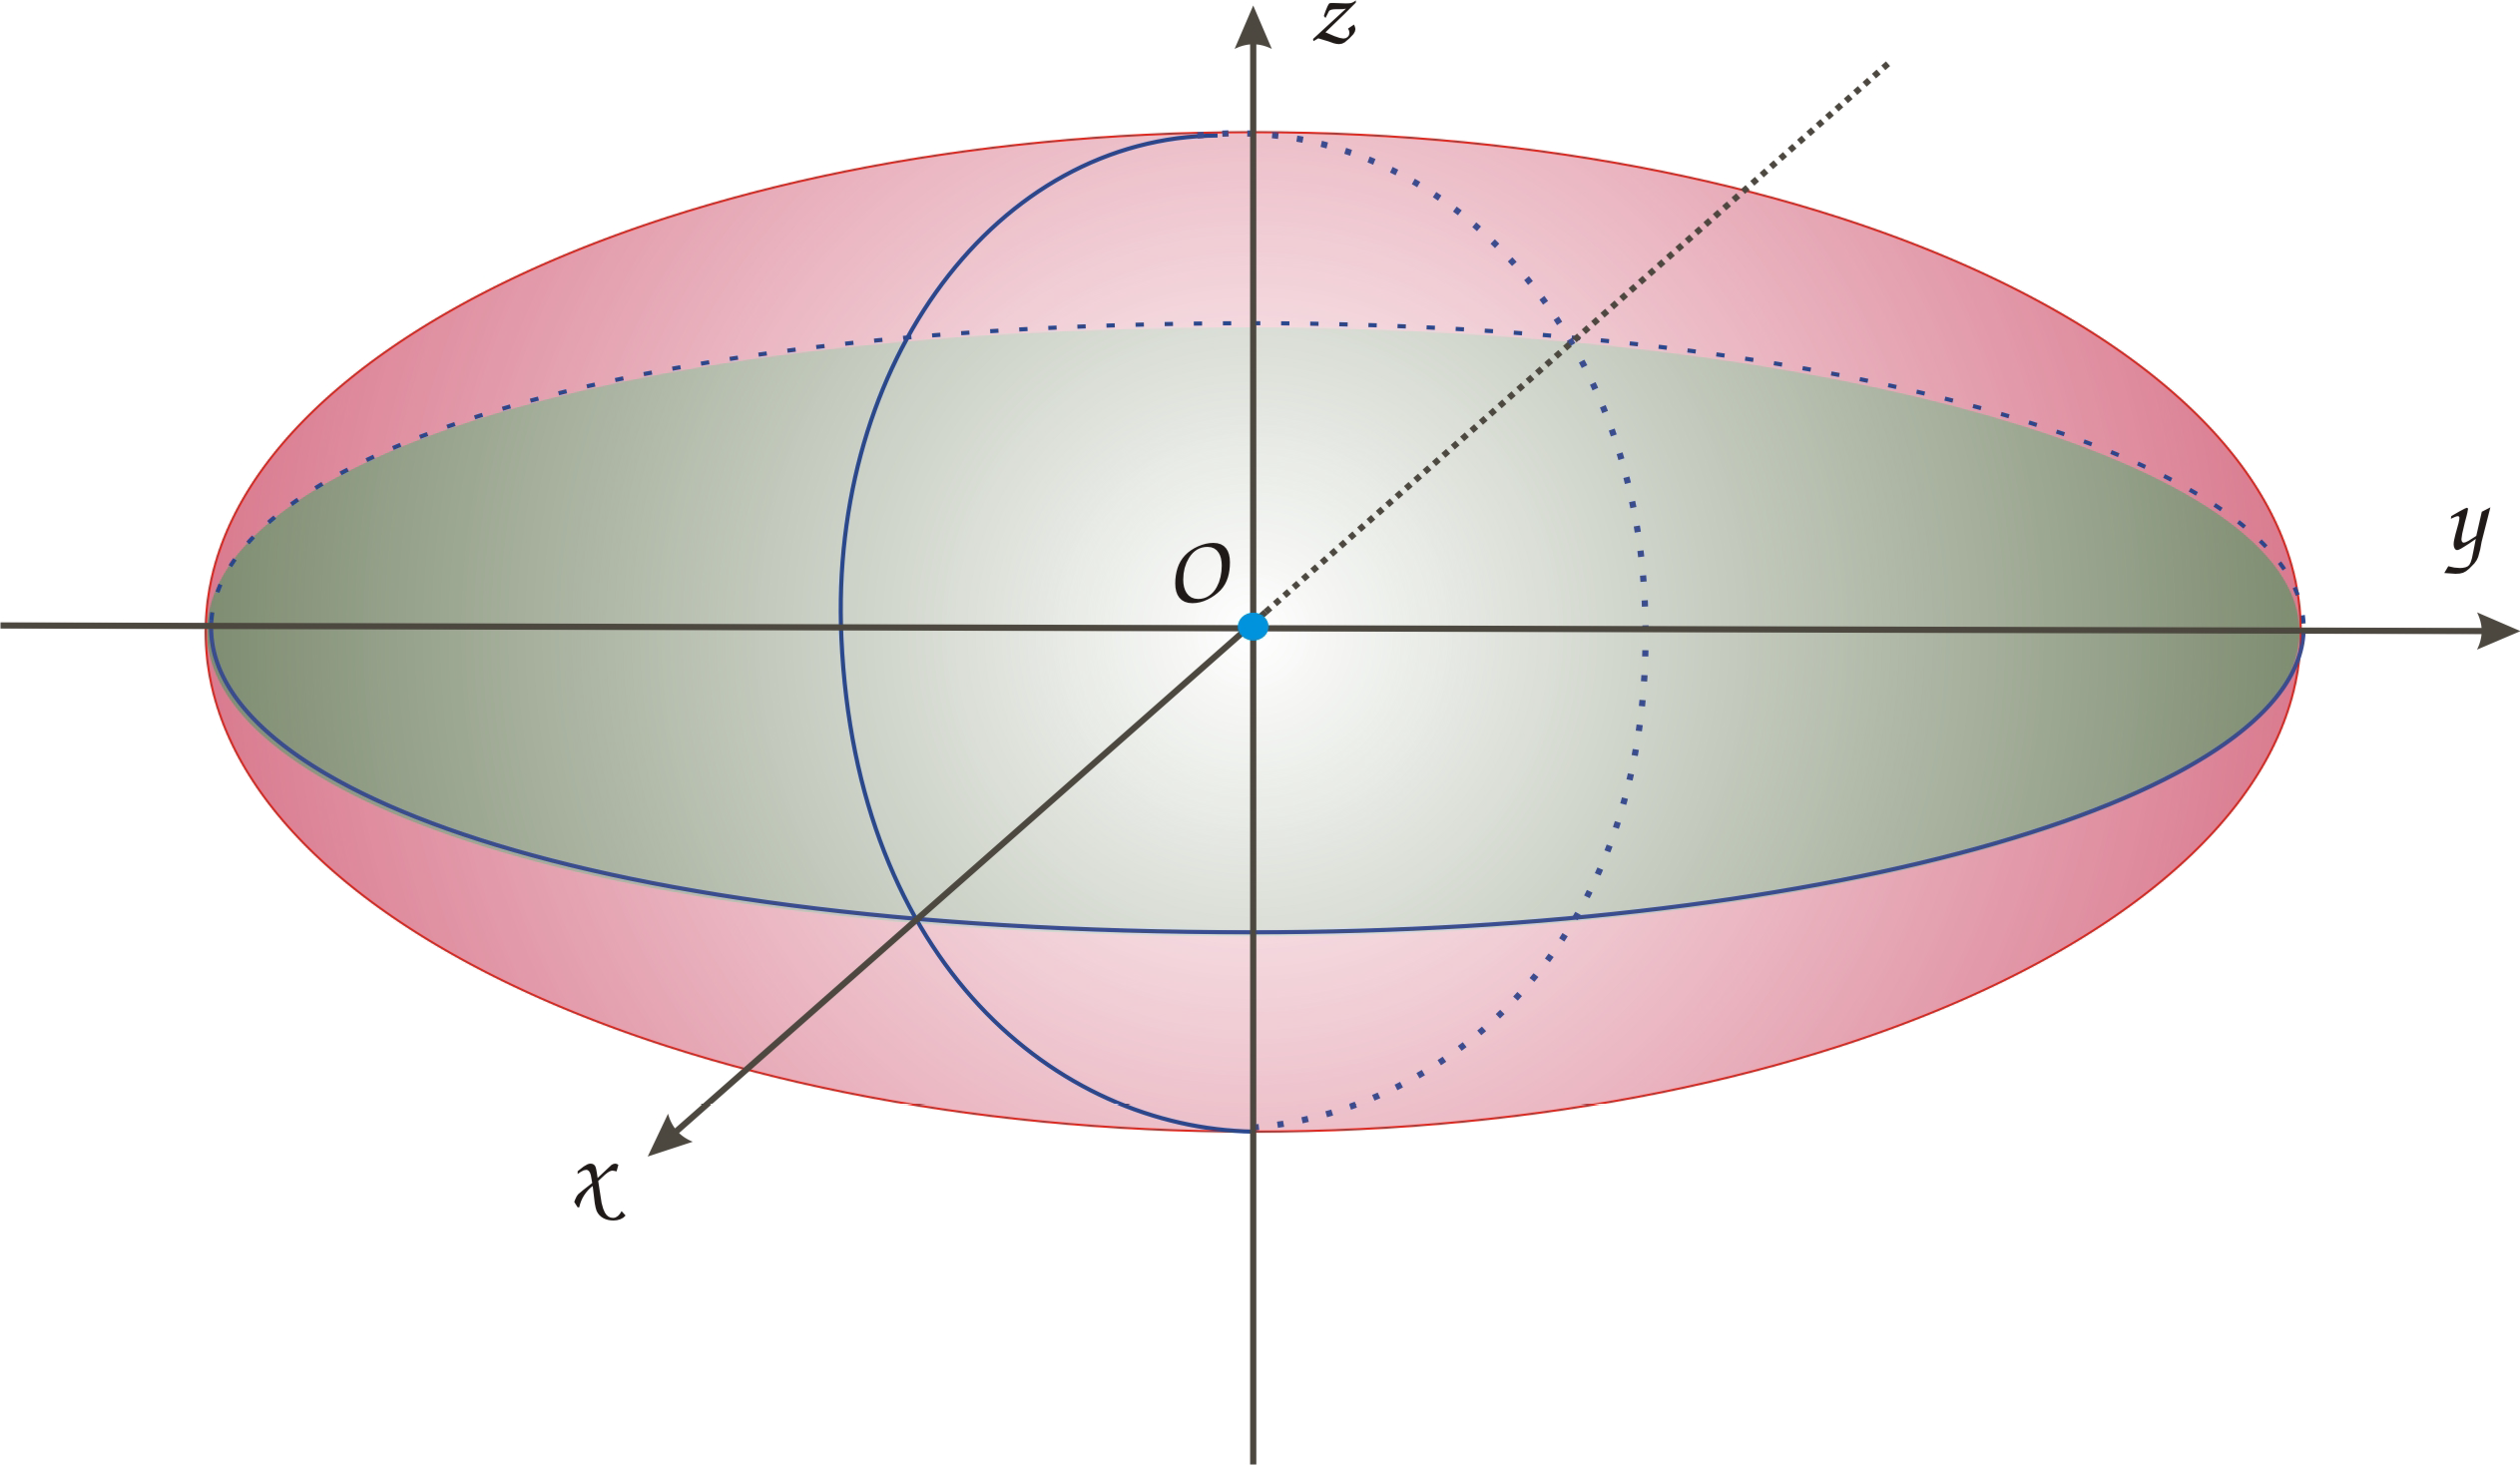
\includegraphics[width = 0.65\textwidth]{./local/image/4.png}
\end{center}
\section{Số nhị phân (Binary):}
\subsection{Các tính chất của số nhị phân}
\begin{itemize}
    \item[-] Số nhị phân n bit có $2^n$ giá trị từ $0$ đến $2^n-1$.
    \item[-] Số nhị phân có giá trị $2^n-1$: $1\cdots \cdots \cdots 1$ (n bit 1) và giá trị $2^n$: $1 \ 0 \cdots \cdots \cdots 0$ (n bit 0).
    \item[-] Số nhị phân có giá trị lẻ là số có LSB = 1; ngược lại giá trị chẵn là số có LSB = 0.
    \item[-] Các bội số của bit:
\end{itemize}
\begin{center}
    1 B (Byte) = 8 bit \\
    1 KB = $2^{10}$ B \\
    1 MB = $2^{10}$ KB \\
    1 GB = $2^{10}$ MB 
\end{center}
\subsection{Các phép toán số học trên số nhị phân:}
\noindent\textbf{a. Phép cộng}
\begin{center}
    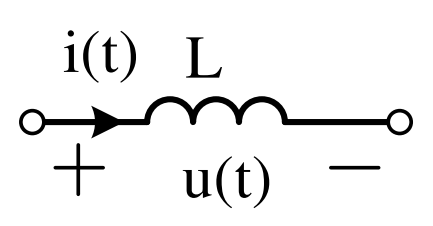
\includegraphics[width = 0.65\textwidth]{./local/image/5.png}
\end{center}
\textbf{b. Phép trừ}
\begin{center}
    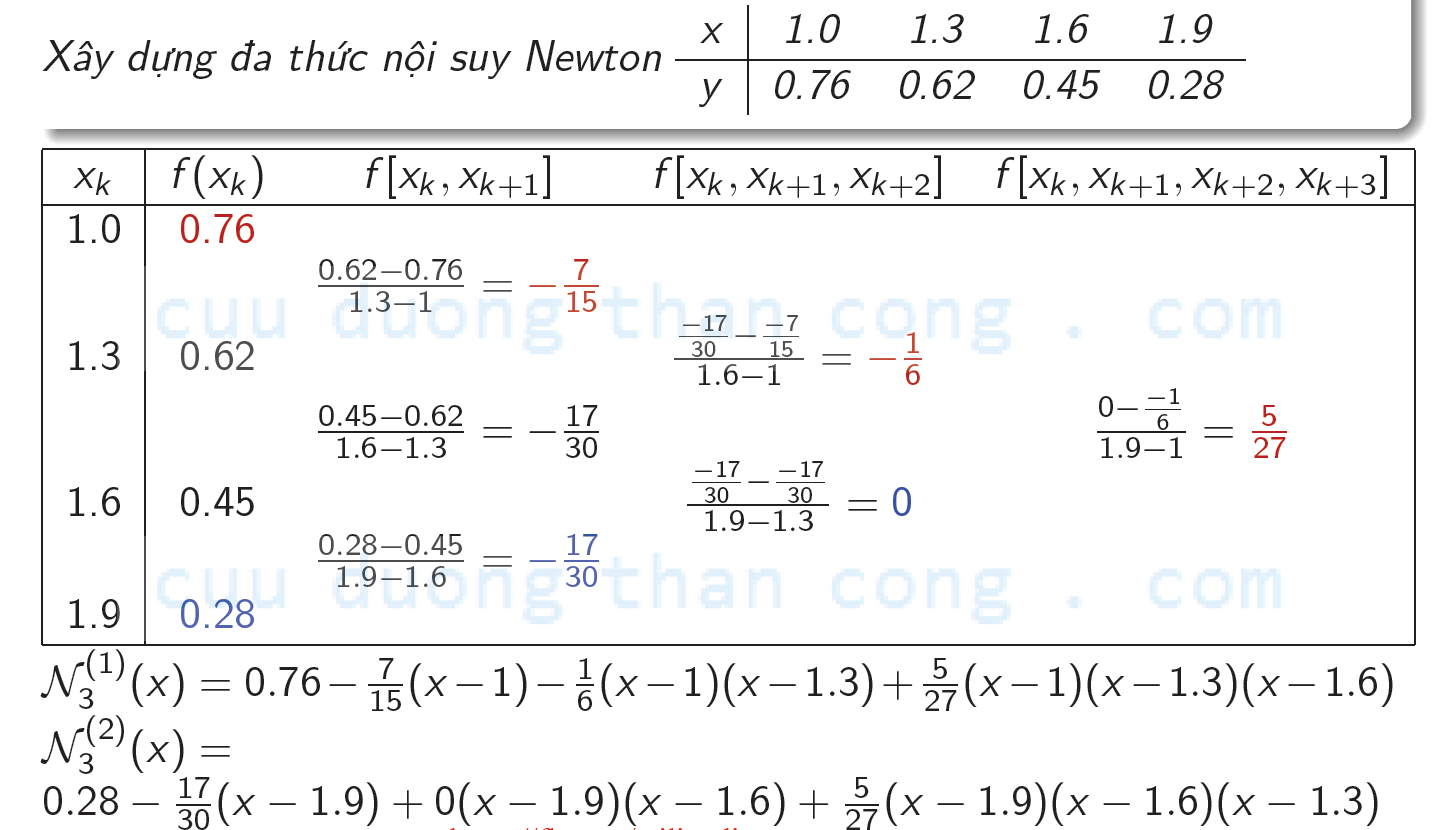
\includegraphics[width = 0.65\textwidth]{./local/image/6.png}
\end{center}
\textbf{c. Phép nhân}
\begin{center}
    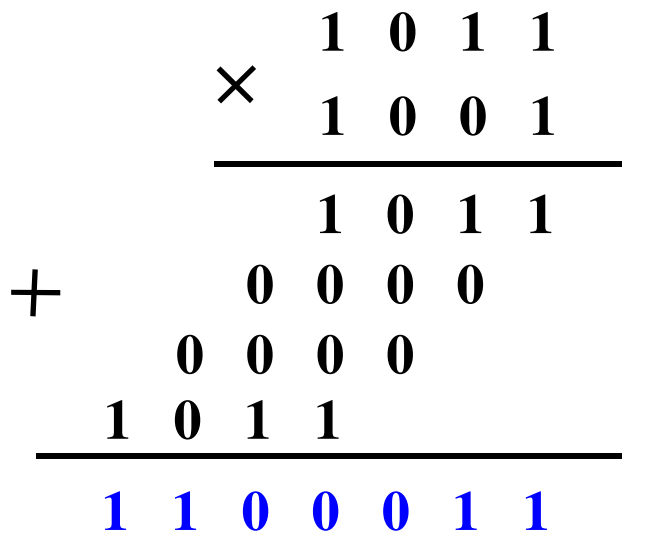
\includegraphics[width = 0.35\textwidth]{./local/image/7.png}
\end{center}
\textbf{d. Phép chia}
\begin{center}
    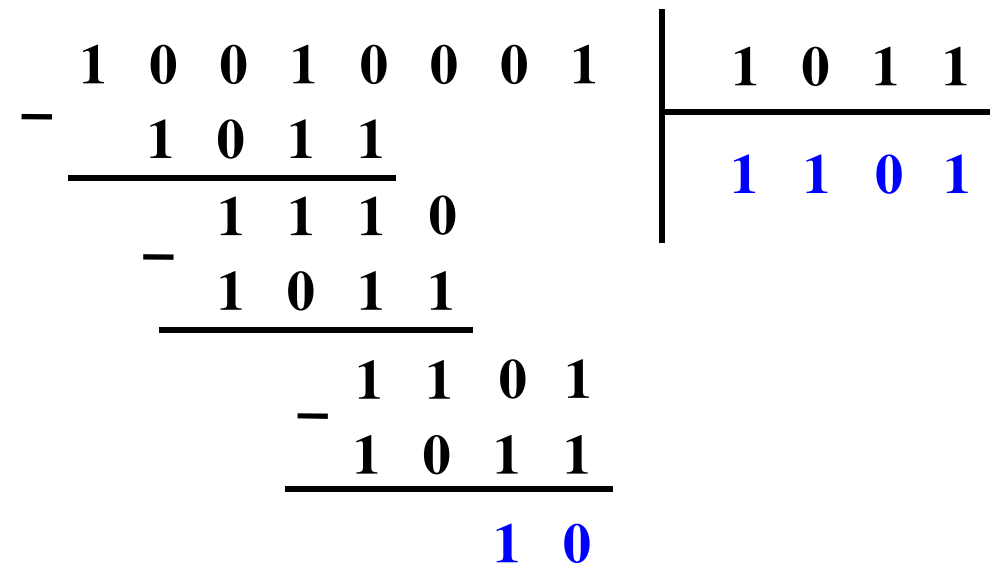
\includegraphics[width = 0.45\textwidth]{./local/image/8.png}
\end{center}
\subsection{Mã nhị phân:}
\textit{\textbf{Từ mã:}} là các tổ hợp nhị phân được sử dụng trong loại mã nhị phân.\\
\textbf{a. Mã nhị phân cho số thập phân (BCD - Binary Coded Decimal)}
\newpage
\section{ĐẠI SỐ BOOLE - CỔNG LOGIC}
\subsection{Cấu trúc đại số Boole:}
Là cấu trúc đại số được định nghĩa trên tập 1 phần tử nhị phân B $=\lbrace 0,1\rbrace$ và các phép toán nhị phân: AND(.), OR(+), NOT(').
\begin{table}[h!]
    \centering
    \begin{tabular}{|cc|c|}
    \hline
    \textbf{x} & \textbf{y} & \textbf{x.y (x AND y)} \\ \hline
    0          & 0          & 0                      \\ 
    0          & 1          & 0                      \\ 
    1          & 0          & 0                      \\ 
    1          & 1          & 1                      \\ \hline
    \end{tabular}
    \qquad \qquad
    \begin{tabular}{|cc|c|}
    \hline
    \textbf{x} & \textbf{y} & \textbf{x+y (x OR y)} \\ \hline
    0          & 0          & 0                     \\ 
    0          & 1          & 1                     \\ 
    1          & 0          & 1                     \\ 
    1          & 1          & 1                     \\ \hline
    \end{tabular}
\end{table}
\begin{table}[h!]
    \centering
    \begin{tabular}{|c|c|}
    \hline
    \textbf{x} & \textbf{x' (NOT x, $\overline{x}$)} \\ \hline
    0          & 1                                   \\ 
    1          & 0                                   \\ \hline
    \end{tabular}
\end{table}

\textbf{*Thứ tự phép toán:} theo thứ tự dấu ngoặc (), NOT, AND, OR.
\subsubsection{Các tiên đề (Axioms):}
\textbf{a. Tính kín (Closure Property)}

\textbf{b. Phần tử đồng nhất (Identity Element):}
\[
    x.1 = 1.x = x 
\]
\[
    x+0 = 0+x = x
\]

\textbf{c. Tính giao hoán (Commutative Property):}
\[
    x.y = y.x
\]
\[
    x+y = y+x
\]

\textbf{d. Tính phân bố (Complement Element):}
\[
    x.(y+z) = x.y + x.z
\]
\[
    x+(y.z)=(x+y)(x+z)
\]

\textbf{e. Phần tử bù (Complement Element):}
\[
    x+\overline{x}=1 \qquad x.\overline{x} = 0
\]
\subsubsection{Các định lý cơ bản (Basic Theorems):}
\textbf{a. Định lý 1:} $\overline{\overline{x}} = x$

\textbf{b. Định lý 2:} $x+x = x \qquad x.x=x$

\textbf{c. Định lý 3:} $x+1=1 \qquad x.0 = 0$

\textbf{d. Định lý 4:} Định lý hấp thu (Absorption)
\[
    x+x.y = x \qquad x.(x+y) = x
\]

\textbf{e. Định lý 5:} Định lý kết hợp (Associative)
\[
    x+(y+z) = (x+y) + z \qquad x.(y.z) = (x.y).z
\]

\textbf{f. Định lý 6:} Định lý De Morgan
\[
    \overline{x+y} = \overline{x}.\overline{y} \qquad \overline{x.y} = \overline{x}+\overline{y}
\]
\subsection{Hàm Boole (Boolean Function):}
\subsubsection{Định nghĩa:}
\begin{itemize}
    \item Hàm Boole là 1 biểu thức được tạo bởi các biến nhị phân và các phép toán nhị phân NOT, AND, OR.
        \[
            F(x,y,z)=x.y+\overline{x}.\overline{y}.z
        \]
    \item Với giá trị cho trước của các biến, hàm Boole sẽ có giá trị là 0 hoặc 1.
    \item Bảng giá trị:
\end{itemize}
\begin{table}[h!]
    \centering
    \begin{tabular}{|ccc|c|}
    \hline
    \textbf{x} & \textbf{y} & \textbf{z} & \textbf{F} \\ \hline
    0          & 0          & 0          & 0          \\ 
    0          & 0          & 1          & 1          \\ 
    0          & 1          & 0          & 0          \\ 
    0          & 1          & 1          & 0          \\ 
    1          & 0          & 0          & 0          \\ 
    1          & 0          & 1          & 0          \\ 
    1          & 1          & 0          & 1          \\ 
    1          & 1          & 1          & 1          \\ \hline
    \end{tabular}
    \end{table}
\subsubsection{Bù của 1 hàm:}
\begin{itemize}
    \item[-] Sử dụng định lý De Morgan:
        \[
            F = x.y+\overline{x}.\overline{y}.z
        \]
        \[
            \overline{F} = \overline{x.y+\overline{x}.\overline{y}.z} = \overline{(x.y)}.\overline{(\overline{x}.\overline{y}.z)}
        \]
        \[
            \overline{F} = (\overline{x} + \overline{y}).(x+y+\overline{z})
        \]
    \item[-] Lấy biểu thức đối ngẫu và lấy bù các biến: Tính đối ngẫu (Duality): Hai biểu thức được gọi là đối ngẫu của nhau khi thay phép toán AND bằng OR, phép toán OR bằng AND, 0 thành 1 và 1 thành 0.
        \[
            F = x.y+\overline{x}.\overline{y}.z
        \]
    Lấy đối ngẫu: $(x.y)(\overline{x}.\overline{y}.z)$

    Bù các biến: $\overline{F} = (\overline{x} + \overline{y}).(x+y+\overline{z})$
\end{itemize}
\subsection{Dạng chính tắc và dạng chuẩn của hàm Boole:}
\subsubsection{Các tích chuẩn (minterm) và tổng chuẩn (Maxterm):}
\begin{itemize}
    \item[-] Tích chuẩn (minterm): $m_i \ (0 \leq i \leq 2^n - 1)$ là các số hạng tích (AND) của n biến mà hàm Boole phụ thuộc với quy ước biến đó có bù nếu nó là 0 và không bù nếu nó là 1.
    \item[-] Tổng chuẩn (Maxterm): $M_i \ (0 \leq i \leq 2^n - 1)$ là các số hạng tổng (OR) của n biến mà hàm Boole phụ thuộc với quy ước biến đó có bù nếu nó là 1 và không bù nếu nó là 0.
\end{itemize}
\begin{table}[h!]
    \centering
    \begin{tabular}{|ccc|c|c|}
    \hline
    \textbf{x} & \textbf{y} & \textbf{z} & \textit{\textbf{minterm}} & \textit{\textbf{Maxterm}} \\ \hline
    0 & 0 & 0 & $m_0 = \overline{x}\ \overline{y}\ \overline{z}$ & $M_0 = x+y+z$ \\ 
    0 & 0 & 1 & $m_1 = \overline{x}\ \overline{y}\ z$            & $M_1 = x+y+\overline{z}$ \\ 
    0 & 1 & 0 & $m_2 = \overline{x}\ y\ \overline{z}$            & $M_2 = x+\overline{y}+z$ \\ 
    0 & 1 & 1 & $m_3 = \overline{x}\ y\ z$                       & $M_3 = x+\overline{y}+\overline{z}$ \\ 
    1 & 0 & 0 & $m_4 = x\ \overline{y}\ \overline{z}$            & $M_4 = \overline{x}+y+z$ \\ 
    1 & 0 & 1 & $m_5 = x\ \overline{y}\ z$                       & $M_5 = \overline{x}+y+\overline{z}$ \\ 
    1 & 1 & 0 & $m_6 = x\ y\ \overline{z}$                       & $M_6 = \overline{x}+\overline{y}+z$ \\ 
    1 & 1 & 1 & $m_7 = x\ y\ z$                                  & $M_7 = \overline{x} + \overline{y} + \overline{z}$ \\ \hline
    \end{tabular}
    \qquad \qquad $m_i = \overline{M_i}$
\end{table}
\newpage
\subsubsection{Dạng chính tắc (Canonical Form):}
\textbf{a. Dạng chính tắc 1:} là dạng tổng của các tích chuẩn (minterm) làm cho hàm Boole có giá trị 1.
\begin{table}[h!]
    \centering
    \begin{tabular}{|ccc|c|}
    \hline
    \textbf{x} & \textbf{y} & \textbf{z} & \textbf{F} \\ \hline
    0          & 0          & 0          & 0          \\ 
    0          & 0          & 1          & 1          \\ 
    0          & 1          & 0          & 1          \\ 
    0          & 1          & 1          & 0          \\ 
    1          & 0          & 0          & 0          \\ 
    1          & 0          & 1          & 1          \\ 
    1          & 1          & 0          & 1          \\ 
    1          & 1          & 1          & 1          \\ \hline
    \end{tabular}
    \qquad
    $\begin{aligned}
        F(x,y,z) &= \overline{x}\ \overline{y}\ z  + \overline{x}\ y\ \overline{z} + x\ \overline{y}\ z + xy\ \overline{z} + xyz \\
                 &= m_1 + m_2 + m_5 + m_6 + m_7 \\
                 &= \varSigma m(1,2,5,6,7) = \varSigma (1,2,5,6,7) \\
        F(x,y,z) &= (x+y+z)(x+ \overline{y} + \overline{z})(\overline{x} + y + z)\\
                 &= M_0 . M_3 . M_4 \\
                 &= \varPi M(0,3,4) = \varPi (0,3,4)
    \end{aligned}$
\end{table}

\textbf{b. Dạng chính tắc 2:} là dạng tích của các tổng chuẩn (Maxterm) làm cho hàm Boole có giá trị 0.

\textbf{TRƯỜNG HỢP HÀM BOOLE TÙY ĐỊNH (don't care):} Hàm Boole n biến có thể không được định nghĩa hết tất cả $2^n$ tổ hợp của n biến phụ thuộc. Khi đó tại các tổ hợp không sử dụng này, hàm Boole sẽ nhận giá trị tùy định (don't care), nghĩa là hàm Boole có thể nhận giá trị 0 hoặc 1.
\begin{table}[h!]
    \centering
    \begin{tabular}{|ccc|c|}
    \hline
    \textbf{x} & \textbf{y} & \textbf{z} & \textbf{F} \\ \hline
    0          & 0          & 0          & X          \\ 
    0          & 0          & 1          & 1          \\ 
    0          & 1          & 0          & 1          \\ 
    0          & 1          & 1          & 0          \\ 
    1          & 0          & 0          & 0          \\ 
    1          & 0          & 1          & 1          \\ 
    1          & 1          & 0          & 1          \\ 
    1          & 1          & 1          & X          \\ \hline
    \end{tabular}
    \qquad
    $\begin{aligned}
        F(x,y,z) &= \varSigma (1,2,5,6) + d(0,7)\\
                 &= \varPi (3,4). D(0,7)
    \end{aligned}$
\end{table}
\subsubsection{Dạng chuẩn (Standard Form):}
\textbf{a. Dạng chuẩn 1:} là dạng tổng các tích (S.O.P - Sum of Product)
\[
    F(x,y,z) = xy + z
\]
\[
    \begin{aligned}
        F(x,y,z) &= xy + z\\
                 &= xy(\overline{z}+z) + (\overline{x}+x)(\overline{y}+y)z\\
                 &= xy\overline{z} + xyz + \overline{x}\ \overline{y} z + \overline{x}\ yz + x\overline{y}\ z + xyz\\
                 &= m_6 + m_7 + m_1 + m_5+ m_3\\
                 &= \varSigma (1,3,5,6,7)\\
        F(x,y,z) &= xy + z\\
                 &= (x+z)(y+z)\\
                 &= (x + \overline{y}\ y + z)(\overline{x}\ x + y +z)\\
                 &= (x + \overline{y} + z)(x+y+z)(\overline{x} + y + z)(x+y+z)\\
                 &= M_2.M_0.M_4\\
                 &= \varPi (0,2,4)
    \end{aligned}
\]
\textbf{b. Dạng chuẩn 2:} là dạng tích các tổng (P.O.S - Product of Sum)
\[
    F(x,y,z) =(x+\overline{z})\overline{y}
\]
\[
    \begin{aligned}
        F(x,y,z) &= (x+\overline{z})\overline{y} = x\overline{y} + \overline{y}\ \overline{z}\\
                 &= x\overline{y}(\overline{z} + z) + (\overline{x} + x)\overline{y}\ \overline{z}\\
                 &= x\overline{y}\ \overline{z} + x\overline{y}\ z + \overline{x}\ \overline{y}\ \overline{z} + x\overline{y}\ \overline{z} \\
                 &= m_4  + m_5 + m_0\\
                 &= \varSigma (0,4,5)\\
        F(x,y,z) &= (x+\overline{z})\overline{y}\\
                 &= (x + \overline{y}\ y + \overline{z})(\overline{x}\ x + \overline{y} + \overline{z}\ z)\\
                 &= (x + \overline{y} + \overline{z})(x + y + \overline{z})\\
                 &= (\overline{x} + \overline{y} + \overline{z})(\overline{x} + \overline{y} + z)(x+\overline{y}+\overline{z})(x + \overline{y} + z)\\
                 &= M_3.M_1.M_7.M_6.M_2\\
                 &= \varPi (1,2,3,6,7)
    \end{aligned}
\]
\subsection{Cổng logic}
\subsubsection{Cổng NOT:}
\begin{center}
    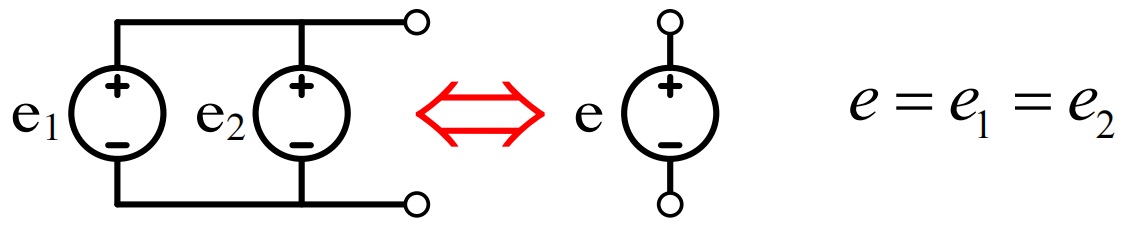
\includegraphics[width = 0.7\textwidth]{./local/image/20.png}
\end{center}
\subsubsection{Cổng AND:}
\begin{center}
    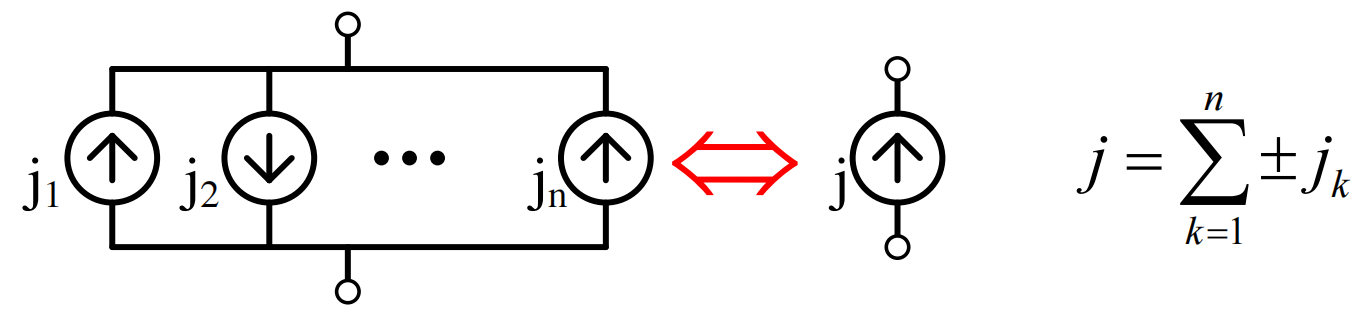
\includegraphics[width = 0.7\textwidth]{./local/image/21.png}
\end{center}
\begin{table}[h!]
    \centering
    \begin{tabular}{|cc|c|}
    \hline
    \textbf{x} & \textbf{y} & \textbf{z} \\ \hline
    0          & 0          & 0                      \\ 
    0          & 1          & 0                      \\ 
    1          & 0          & 0                      \\ 
    1          & 1          & 1                      \\ \hline
    \end{tabular} \qquad 
    $\begin{aligned}
        &\text{Với cổng AND có nhiều ngõ vào,}\\
        &\text{ngõ ra sẽ là 1 nếu tất cả các ngõ vào đều là 1}
    \end{aligned}$
\end{table}
\subsubsection{Cổng OR:}
\begin{center}
    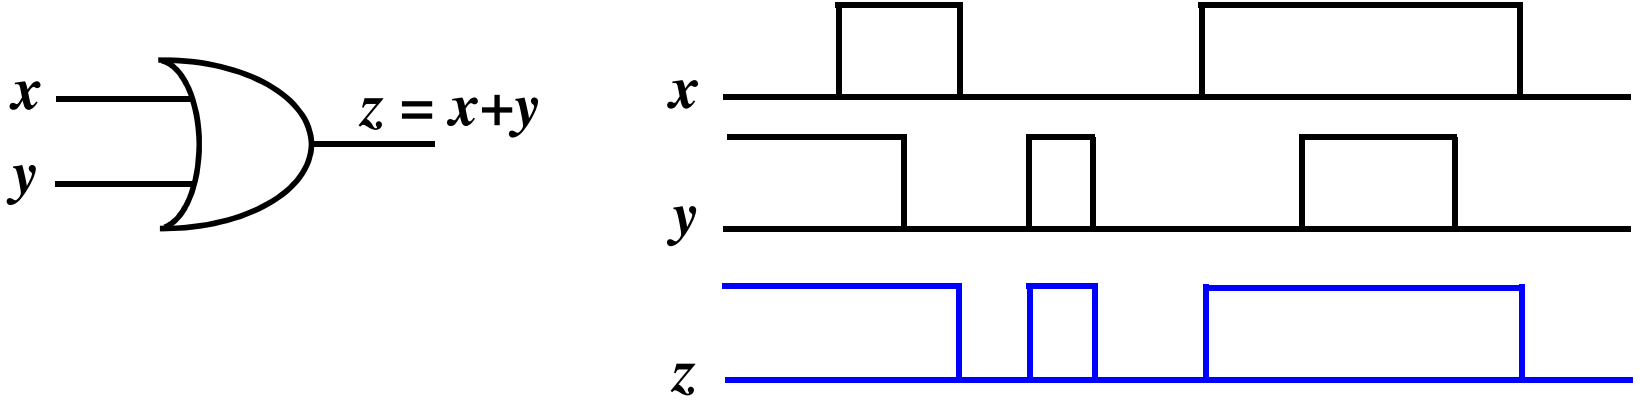
\includegraphics[width = 0.7\textwidth]{./local/image/22.png}
\end{center}
\begin{table}[h!]
    \centering
    \begin{tabular}{|cc|c|}
    \hline
    \textbf{x} & \textbf{y} & \textbf{z} \\ \hline
    0          & 0          & 0                      \\ 
    0          & 1          & 1                      \\ 
    1          & 0          & 1                      \\ 
    1          & 1          & 1                      \\ \hline
    \end{tabular} \qquad 
    $\begin{aligned}
        &\text{Với cổng OR có nhiều ngõ vào,}\\
        &\text{ngõ ra sẽ là 0 nếu tất cả các ngõ vào đều là 0}
    \end{aligned}$
\end{table}
\subsubsection{Cổng NAND:}
\begin{center}
    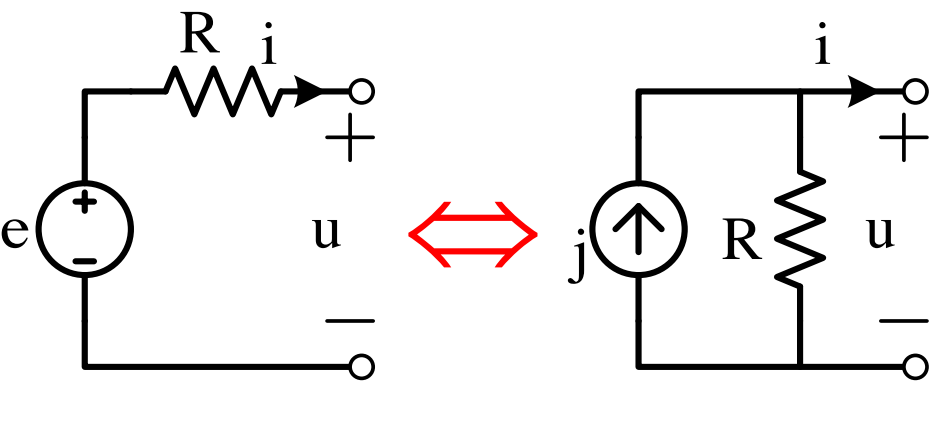
\includegraphics[width = 0.7\textwidth]{./local/image/23.png}
\end{center}
\begin{table}[h!]
    \centering
    \begin{tabular}{|cc|c|}
    \hline
    \textbf{x} & \textbf{y} & \textbf{z} \\ \hline
    0          & 0          & 1                      \\ 
    0          & 1          & 1                      \\ 
    1          & 0          & 1                      \\ 
    1          & 1          & 0                      \\ \hline
    \end{tabular} \qquad 
    $\begin{aligned}
        &\text{Với cổng NAND có nhiều ngõ vào,}\\
        &\text{ngõ ra sẽ là 0 nếu tất cả các ngõ vào đều là 1}
    \end{aligned}$
\end{table}
\subsubsection{Cổng NOR:}
\begin{center}
    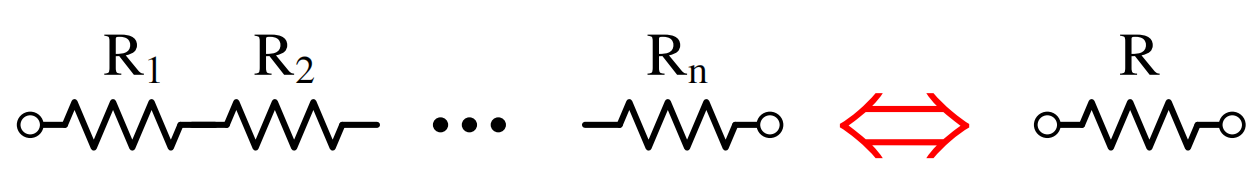
\includegraphics[width = 0.7\textwidth]{./local/image/24.png}
\end{center}
\begin{table}[h!]
    \centering
    \begin{tabular}{|cc|c|}
    \hline
    \textbf{x} & \textbf{y} & \textbf{z} \\ \hline
    0          & 0          & 1                      \\ 
    0          & 1          & 0                      \\ 
    1          & 0          & 0                      \\ 
    1          & 1          & 0                      \\ \hline
    \end{tabular} \qquad 
    $\begin{aligned}
        &\text{Với cổng NOR có nhiều ngõ vào,}\\
        &\text{ngõ ra sẽ là 1 nếu tất cả các ngõ vào đều là 0}
    \end{aligned}$
\end{table}
\subsubsection{Cổng XOR:}
\begin{center}
    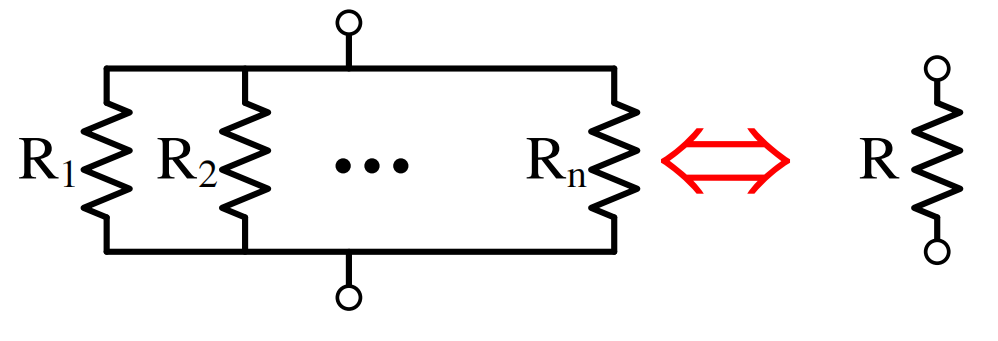
\includegraphics[width = 0.7\textwidth]{./local/image/25.png}
\end{center}
\begin{table}[h!]
    \centering
    \begin{tabular}{|cc|c|}
    \hline
    \textbf{x} & \textbf{y} & \textbf{z} \\ \hline
    0          & 0          & 0                      \\ 
    0          & 1          & 1                      \\ 
    1          & 0          & 1                      \\ 
    1          & 1          & 0                      \\ \hline
    \end{tabular} \qquad 
    $\begin{aligned}
        &\text{Với cổng XOR có nhiều ngõ vào, ngõ ra sẽ là 1}\\
        &\text{ếu tổng số bit 1 ở các ngõ vào là số lẻ}
    \end{aligned}$
\end{table}
\[
    z = x \oplus y = \overline{x}\ y + x\ \overline{y} = (x+y)(\overline{x} + \overline{y})
\]
\subsubsection{Cổng XNOR:}
\begin{center}
    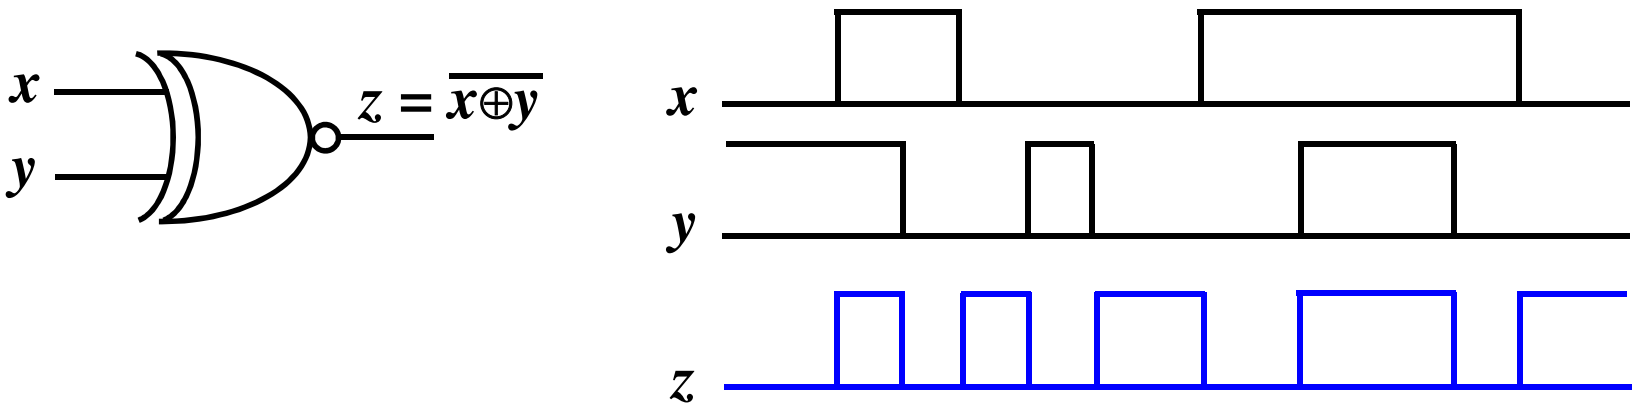
\includegraphics[width = 0.7\textwidth]{./local/image/26.png}
\end{center}
\begin{table}[h!]
    \centering
    \begin{tabular}{|cc|c|}
    \hline
    \textbf{x} & \textbf{y} & \textbf{z} \\ \hline
    0          & 0          & 1                      \\ 
    0          & 1          & 0                      \\ 
    1          & 0          & 0                      \\ 
    1          & 1          & 1                      \\ \hline
    \end{tabular} \qquad 
    $\begin{aligned}
        &\text{Với cổng XNOR có nhiều ngõ vào, ngõ ra sẽ là 1}\\
        &\text{nếu tổng số bit 1 ở các ngõ vào là số chẵn}
    \end{aligned}$
\end{table}
\[
    z = \overline{x \oplus y} = \overline{x}\ \overline{y} +xy = (x+\overline{y})(\overline{x} + y)
\]
\newpage
\section{HỆ TỔ HỢP}
\subsection{Giới thiệu - Cách thiết kế hệ tổ hợp:}
\subsection{Bộ cộng - trừ nhị phân:}
\subsubsection{Bộ cộng (Adder):}
\subsubsection{Bộ trừ (Subtractor):}
\subsubsection{Bộ cộng/trừ nhị phân song song:}
\subsection{Hệ chuyển mã (Code conversion):}
\subsection{Bộ giải mã (Decoder):}
\subsubsection{Giới thiệu:}
\subsubsection{IC giải mã:}
\subsubsection{Sử dụng bộ giải mã thực hiện hàm Boole:}
\subsection{Bộ mã hóa (Encoder):}
\subsubsection{Giới thiệu:}
\subsubsection{IC mã hóa ưu tiên $8 \to 3$ (74148):}
\subsection{Bộ dồn kênh (Multiplexer - MUX):}
\subsubsection{Giới thiệu:}
\subsubsection{IC dồn kênh:}
\subsubsection{Sử dụng bộ MUX thực hiện hàm Boole:}
\subsection{Bộ ohaan kênh (Demux):}
\subsubsection{Giới thiệu:}
\subsubsection{IC phân kênh 74LS155:}
\subsection{Bộ so sánh độ lớn (Comparator):}
\subsubsection{Giới thiệu:}
\subsubsection{IC so sánh 74LS85:}
\end{document}